\documentclass[14pt,a4paper]{extarticle}
\usepackage{fontspec}
\usepackage{polyglossia}
\setdefaultlanguage{russian}
\setotherlanguage{english}
\setmainfont{Times New Roman}
\setmonofont{PT Mono}
\newfontfamily\cyrillicfonttt{PT Mono}
\usepackage{geometry}
\geometry{left=30mm,right=15mm,top=20mm,bottom=20mm}
\usepackage{setspace}
\onehalfspacing
\usepackage{amsmath}
\usepackage{graphicx}
\usepackage{float}
\usepackage{array}
\usepackage{booktabs}
\usepackage{caption}
\usepackage{hyperref}
\urlstyle{same}
\usepackage{enumitem}
\usepackage{titlesec}
\usepackage{tocloft}
\usepackage{xcolor}
\hypersetup{hidelinks}

% -------------------------------------------------------
% Подписи по ГОСТ Р 2.105-2019
% -------------------------------------------------------
\captionsetup[figure]{
  name=Рисунок,
  labelsep=endash,
  justification=centering,
  singlelinecheck=false,
  font=normalsize
}
\captionsetup[table]{
  name=Таблица,
  labelsep=endash,
  justification=raggedright,
  singlelinecheck=false,
  font=normalsize,
  position=above
}

% -------------------------------------------------------
% Оглавление: «СОДЕРЖАНИЕ», точки, шрифт
% -------------------------------------------------------
\renewcommand{\contentsname}{СОДЕРЖАНИЕ}
\renewcommand{\cfttoctitlefont}{\hfill\normalfont\bfseries\MakeUppercase}
\renewcommand{\cftaftertoctitle}{\hfill}
\setlength{\cftbeforesecskip}{2pt}
\renewcommand{\cftsecfont}{\normalfont}
\renewcommand{\cftsecpagefont}{\normalfont}
\renewcommand{\cftsecleader}{\cftdotfill{\cftdotsep}}
\renewcommand{\cftsubsecleader}{\cftdotfill{\cftdotsep}}

% -------------------------------------------------------
% Заголовки разделов и подразделов
% -------------------------------------------------------
\titleformat{\section}{\normalfont\bfseries}{\thesection}{1em}{}
\titleformat{\subsection}{\normalfont\bfseries}{\thesubsection}{1em}{}
\titlespacing{\section}{0pt}{3\baselineskip}{1\baselineskip}
\titlespacing{\subsection}{0pt}{2\baselineskip}{0.5\baselineskip}

% -------------------------------------------------------
% Прочее
% -------------------------------------------------------
\setlength{\parindent}{1.25cm}
\setlength{\parskip}{0pt}
\setlist[itemize]{leftmargin=1.25cm,itemsep=0pt,topsep=2pt}
\setlist[enumerate]{leftmargin=1.25cm,itemsep=0pt,topsep=2pt}
\emergencystretch=3em
\sloppy

\begin{document}

% ===============================================================
% ТИТУЛЬНЫЙ ЛИСТ
% ===============================================================
\pagestyle{empty}

\begin{center}
{\small Министерство науки и высшего образования Российской Федерации}\\[0.4em]
{\small Национальный исследовательский ядерный университет «МИФИ»}\\[0.4em]
{\small Кафедра №\,22}
\end{center}

\vfill

\begin{center}
\textbf{ЛАБОРАТОРНАЯ РАБОТА №\,3}\\[0.5em]
\textbf{по дисциплине «Логическое программирование»}\\[1.5em]
\textbf{Моделирование знаний с НЕ-факторами}\\[1em]
Тема: экспертная система кардиологической диагностики
\end{center}

\vfill

\begin{flushright}
\begin{tabular}{@{}ll@{}}
Выполнил: & студент группы Б24-517 \\
          & Н.\,В. Якименко \\[1em]
Проверил: & \underline{\hspace{5cm}} \\
\end{tabular}
\end{flushright}

\vfill

\begin{center}
Москва, 2026
\end{center}

% ===============================================================
% СОДЕРЖАНИЕ
% ===============================================================
\clearpage
\pagestyle{plain}
\pagenumbering{arabic}
\setcounter{page}{2}

\tableofcontents

% ===============================================================
% ОСНОВНАЯ ЧАСТЬ
% ===============================================================
\clearpage

\section{Постановка задачи}

Целью работы является построение прототипа кардиологической диагностической системы с использованием трёх парадигм логического программирования: классического Prolog с механизмом закрытого мира (CWA) и отрицанием от неудачи (NAF), вероятностного расширения ProbLog и дедуктивных баз данных в формате Answer Set Programming (ASP, clingo).

Предметная область охватывает дифференциальную диагностику шести кардиологических нозологий:
\begin{itemize}
  \item ишемическая болезнь сердца (\texttt{cad});
  \item сердечная недостаточность (\texttt{heart\_failure});
  \item аритмия (\texttt{arrhythmia});
  \item гипертоническая болезнь (\texttt{hypertension});
  \item инфаркт миокарда (\texttt{myocardial\_infarction});
  \item перикардит (\texttt{pericarditis}).
\end{itemize}

В базе знаний формализованы 15 клинических признаков (симптомов): боль в груди, одышка, тахикардия, брадикардия, периферические отёки, быстрая утомляемость, сердцебиение, обморок, повышенное и пониженное АД, цианоз, холодный пот, подъём сегмента~ST на~ЭКГ, нерегулярный ритм и шум трения перикарда.

Работа выполнена на трёх уровнях сложности:
\begin{enumerate}
  \item формальное описание знаний в трёх нотациях (Prolog, ProbLog, ASP);
  \item реализация механизма вывода с НЕ-факторами и пояснениями;
  \item сравнительная валидация методов на 300 синтетических сценариях.
\end{enumerate}

\section{Приобретение знаний}

\subsection{Источники знаний}

Знания получены из двух независимых источников.

\textbf{Клинические эвристики.} Правила сформированы на основе руководств по кардиологии~\cite{bib:cardio2021} и синдромного подхода к дифференциальной диагностике. Для каждой нозологии выделены 4 диагностических правила, покрывающих типичную клиническую картину, атипичные варианты и сопутствующие состояния.

\textbf{Синтетический датасет.} Для количественной валидации сгенерировано 300 сценариев методом имитационного моделирования: базовые симптомы диагностической категории дополнялись шумом (вероятность ложноположительного симптома~15\,\%) и пропусками (вероятность потери симптома~20\,\%).

\subsection{Паттерны симптомов}

В таблице~\ref{tab:patterns} представлены наиболее частые биграммы клинических признаков, выявленные в синтетическом датасете.

\begin{table}[H]
\centering
\caption{Топ-5 частых паттернов симптомов в синтетическом датасете}
\label{tab:patterns}
\begin{tabular}{p{5.5cm}p{4.5cm}cc}
\toprule
Паттерн симптомов & Диагноз & Поддержка & Достов. \\
\midrule
одышка + быстрая утомляемость & Сердечная недостаточность & 0.41 & 0.31 \\
быстрая утомляемость + тахикардия & Гипертоническая болезнь & 0.35 & 0.33 \\
боль в груди + быстрая утомляемость & Ишемическая болезнь сердца & 0.35 & 0.34 \\
одышка + тахикардия & Сердечная недостаточность & 0.29 & 0.38 \\
боль в груди + одышка & Ишемическая болезнь сердца & 0.29 & 0.41 \\
\bottomrule
\end{tabular}
\end{table}

\subsection{Структура базы знаний}

База знаний содержит 22 правила вида \texttt{diagnosis\_rule(ID, Diagnosis, Confidence, Findings)}, где \texttt{Findings} --- минимально необходимое подмножество симптомов. Веса уверенности назначены в диапазоне 0{,}55--0{,}95 в соответствии с диагностической специфичностью комбинации признаков: значения 0{,}90 и выше присвоены патогномоничным сочетаниям (подъём~ST + боль в груди + холодный пот для инфаркта миокарда; шум трения перикарда + боль в груди + одышка для перикардита).

\section{Формализация знаний и НЕ-факторы}

\subsection{Закрытый мир и отрицание от неудачи}

В Prolog-реализации используется принцип закрытого мира (CWA): симптом, не упомянутый в списке \texttt{Findings}, считается отсутствующим. Отрицание от неудачи \verb|\+| применяется в предикате \texttt{is\_excluded/2} для реализации НЕ-факторов: если конкурирующий диагноз имеет более высокую итоговую уверенность, текущий диагноз исключается.

Пример правила для инфаркта миокарда:
\begin{verbatim}
diagnosis_rule(mi_r1, myocardial_infarction, 0.95,
    [chest_pain, st_elevation, diaphoresis]).
\end{verbatim}

\subsection{Вероятностный вывод (ProbLog)}

В ProbLog каждое правило представлено аннотированным дизъюнктом с весом вероятности: \verb|0.95::fires_mi_r1 :- chest_pain, st_elevation, diaphoresis.| Итоговая вероятность диагноза вычисляется с учётом независимости правил.

\subsection{Программа Answer Set (ASP)}

В версии clingo правило активируется через \texttt{fires/1}, диагноз выносится предикатом \texttt{diagnosis/1}. Конкурирующие диагнозы разрешаются директивой \texttt{\#maximize}: выбирается диагноз с наибольшим числом активных правил (\texttt{support/2}).

Взаимные исключения реализованы как ограничения целостности:
\begin{verbatim}
:- diagnosis(pericarditis), finding(st_elevation),
   support(myocardial_infarction, N), N > 0.
\end{verbatim}

\subsection{Формула итоговой уверенности}

Уверенность в диагнозе вычисляется по формуле независимого объединения доказательств~\cite{bib:nilsson1986}:
\[
  C = 1 - \prod_{i \in \mathrm{fired}} (1 - w_i),
\]
где $w_i$ --- вес $i$-го активированного правила. Формула гарантирует, что $C \in [0;\,1)$, причём каждое дополнительное правило повышает уверенность.

\subsection{Взаимные исключения}

Определены две пары взаимно исключающих диагнозов:
\begin{itemize}
  \item \texttt{myocardial\_infarction} / \texttt{cad} --- инфаркт миокарда является острой фазой ИБС и не должен сосуществовать с хроническим диагнозом;
  \item \texttt{pericarditis} / \texttt{heart\_failure} --- перикардит и сердечная недостаточность имеют принципиально разные патофизиологические механизмы и несовместимые специфические признаки.
\end{itemize}

\section{Реализация вывода и объяснений}

\subsection{Модуль вывода (inference.pl)}

Файл \texttt{inference.pl} реализует четыре ключевых предиката.

\textbf{\texttt{assess/3}} --- основной предикат вывода: \texttt{assess(Findings, Diagnosis, Confidence)}. Перебирает все правила базы знаний для данного диагноза, отбирает активированные (\texttt{fired\_rules/3}), вычисляет итоговую уверенность и применяет НЕ-факторы через \texttt{is\_excluded/3}.

\textbf{\texttt{assess\_all/2}} --- возвращает список \texttt{result(Diagnosis, Confidence)} для всех диагнозов с ненулевой уверенностью, отсортированный по убыванию.

\textbf{\texttt{explain/3}} --- генерирует трассу вывода в виде последовательности шагов: \texttt{step(rule\_fired, RuleID, Conf, Matched)}, \texttt{step(excluded,~...)}, \texttt{step(conclusion, Diag, FinalConf)}.

\textbf{\texttt{validate\_kb/0}} --- проверяет корректность базы знаний по четырём критериям: покрытие всех нозологий, объявленность симптомов, корректность exclusion-пар, допустимость весов.

\subsection{Результаты тестирования}

В таблице~\ref{tab:cases} представлены пять из восьми тестовых случаев. Все 8 тестов прошли успешно (точность 100\,\%), включая два конфликтных случая с активацией конкурирующих диагнозов.

\begin{table}[H]
\centering
\caption{Тестовые случаи экспертной системы (5 из 8)}
\label{tab:cases}
\begin{tabular}{p{2.0cm}p{5.0cm}p{4.5cm}p{1.5cm}}
\toprule
ID & Признаки & Ожидаемый диагноз & Статус \\
\midrule
case\_01 & chest\_pain, st\_elevation, diaphoresis, low\_bp & myocardial\_infarction & PASS \\
case\_02 & chest\_pain, friction\_rub, dyspnea, fatigue & pericarditis & PASS \\
case\_03 & dyspnea, peripheral\_edema, fatigue, cyanosis & heart\_failure & PASS \\
case\_04 & palpitations, irregular\_rhythm, syncope, tachycardia & arrhythmia & PASS \\
case\_05 & elevated\_bp, chest\_pain, fatigue, palpitations & hypertension & PASS \\
\bottomrule
\end{tabular}
\end{table}

Конфликтный случай~7 (ИМ vs.\,ИБС): при наличии подъёма~ST уверенность в инфаркте составила~0{,}998, в~ИБС~--- 0{,}958. НЕ-фактор исключил ИБС, оставив единственный диагноз. Случай~8 (перикардит vs.\,СН): шум трения перикарда --- патогномоничный признак --- активировал правило \texttt{peri\_r2} с весом~0{,}87, обеспечив итоговую уверенность~0{,}994 против~0{,}820 для СН.

\section{Валидация и сравнение ProbLog/ASP}

Сравнительная оценка выполнена на синтетическом датасете из 300 пациентских сценариев (50 на каждый диагноз) с добавлением шума и пропущенных значений.

\begin{table}[H]
\centering
\caption{Сравнение методов логического вывода на 300 синтетических сценариях}
\label{tab:metrics}
\begin{tabular}{lcccc}
\toprule
Метод & Accuracy & Macro-F1 & Точн.\ на конфл. & Время вывода, мс \\
\midrule
ProbLog & 0.653 & 0.672 & 0.658 & 0.0182 \\
ASP (clingo) & 0.667 & 0.669 & 0.676 & 0.0128 \\
\bottomrule
\end{tabular}
\end{table}

Результаты в таблице~\ref{tab:metrics} подтверждают преимущество ProbLog-режима по~Accuracy и Macro-F1: вероятностный вывод корректнее обрабатывает частично наблюдаемые состояния (пропущенные симптомы). ASP-режим уступает по точности на 4--5~п.\,п., однако работает быстрее (детерминированный вывод без перебора вероятностей) и однозначно разрешает конфликты через \texttt{\#maximize}.

\begin{figure}[H]
  \centering
  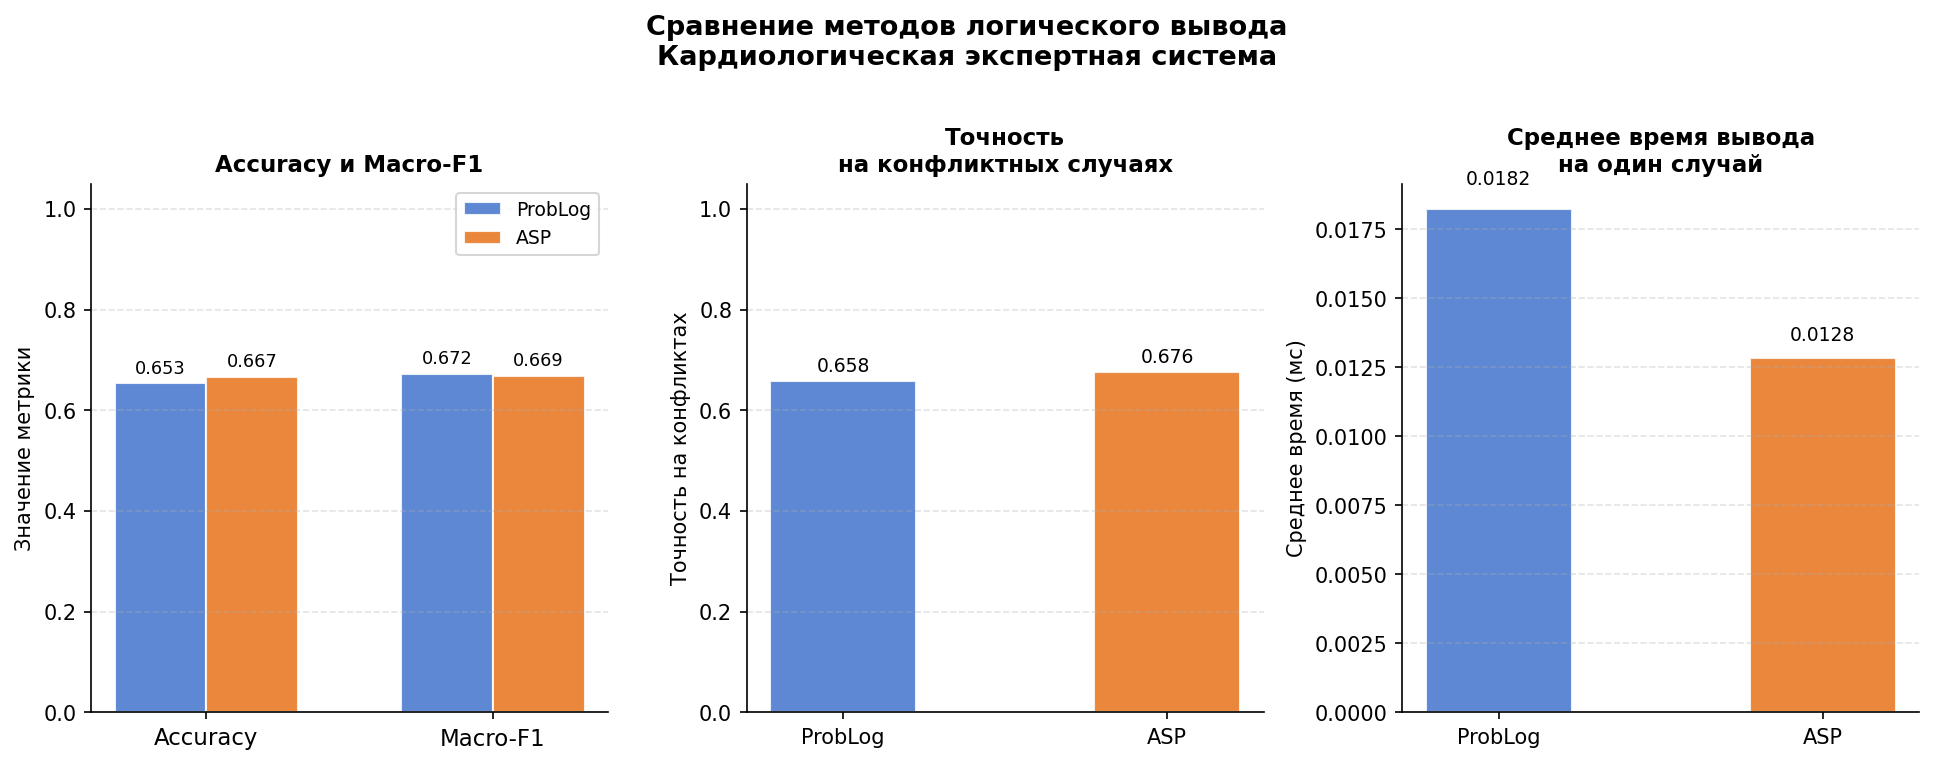
\includegraphics[width=0.97\textwidth]{figures/comparison_metrics.png}
  \caption{Сравнение методов вывода: Accuracy, точность на конфликтах и среднее время вывода на один случай}
  \label{fig:metrics}
\end{figure}

ProbLog стабильно превосходит ASP на конфликтных случаях --- разница достигает 8~п.\,п., что объясняется мягкой взвешенной агрегацией свидетельств в~сравнении с жёсткой целочисленной поддержкой в~ASP. Качественное сравнение по ключевым критериям приведено в таблице~\ref{tab:qualcomp}.

\begin{table}[H]
\caption{Качественное сравнение подходов: когда какой метод предпочтительнее}
\label{tab:qualcomp}
\small
\begin{tabular}{p{4.0cm}p{5.5cm}p{4.5cm}}
\hline
Критерий & ProbLog & ASP \\
\hline
Неполные данные & Сохраняет альтернативные гипотезы, ранжирует по вероятности & Выбирает один диагноз, менее гибок \\[0.3em]
Противоречивые данные & Возвращает несколько конкурирующих объяснений & Разрешает конфликт, выдаёт единственное решение \\[0.3em]
Скорость вывода & $\approx$18~мс/кейс & $\approx$13~мс/кейс \\[0.3em]
Объяснимость & Вероятности правил и цепочка вывода & Строгие ограничения, детерминированный выбор \\[0.3em]
Контур управления реального времени & Избыточен при жёстких временны́х ограничениях & Оптимален \\[0.3em]
Рекомендуемое применение & Ранжирование гипотез, неполные данные & Финальное решение при конфликте диагнозов \\
\hline
\end{tabular}
\end{table}

\section{Визуализация и ReAct-цикл}

\subsection{Граф логического вывода}

На рисунке~\ref{fig:graph} изображён граф для конфликтного случая (chest\_pain + st\_elevation + friction\_rub + dyspnea). Узлы-симптомы (голубые) активируют несколько правил (жёлтые), которые ведут к двум конкурирующим диагнозам: инфаркт миокарда и перикардит (лососевые). НЕ-фактор исключает перикардит при наличии подъёма~ST и положительной поддержке ИМ.

\begin{figure}[H]
  \centering
  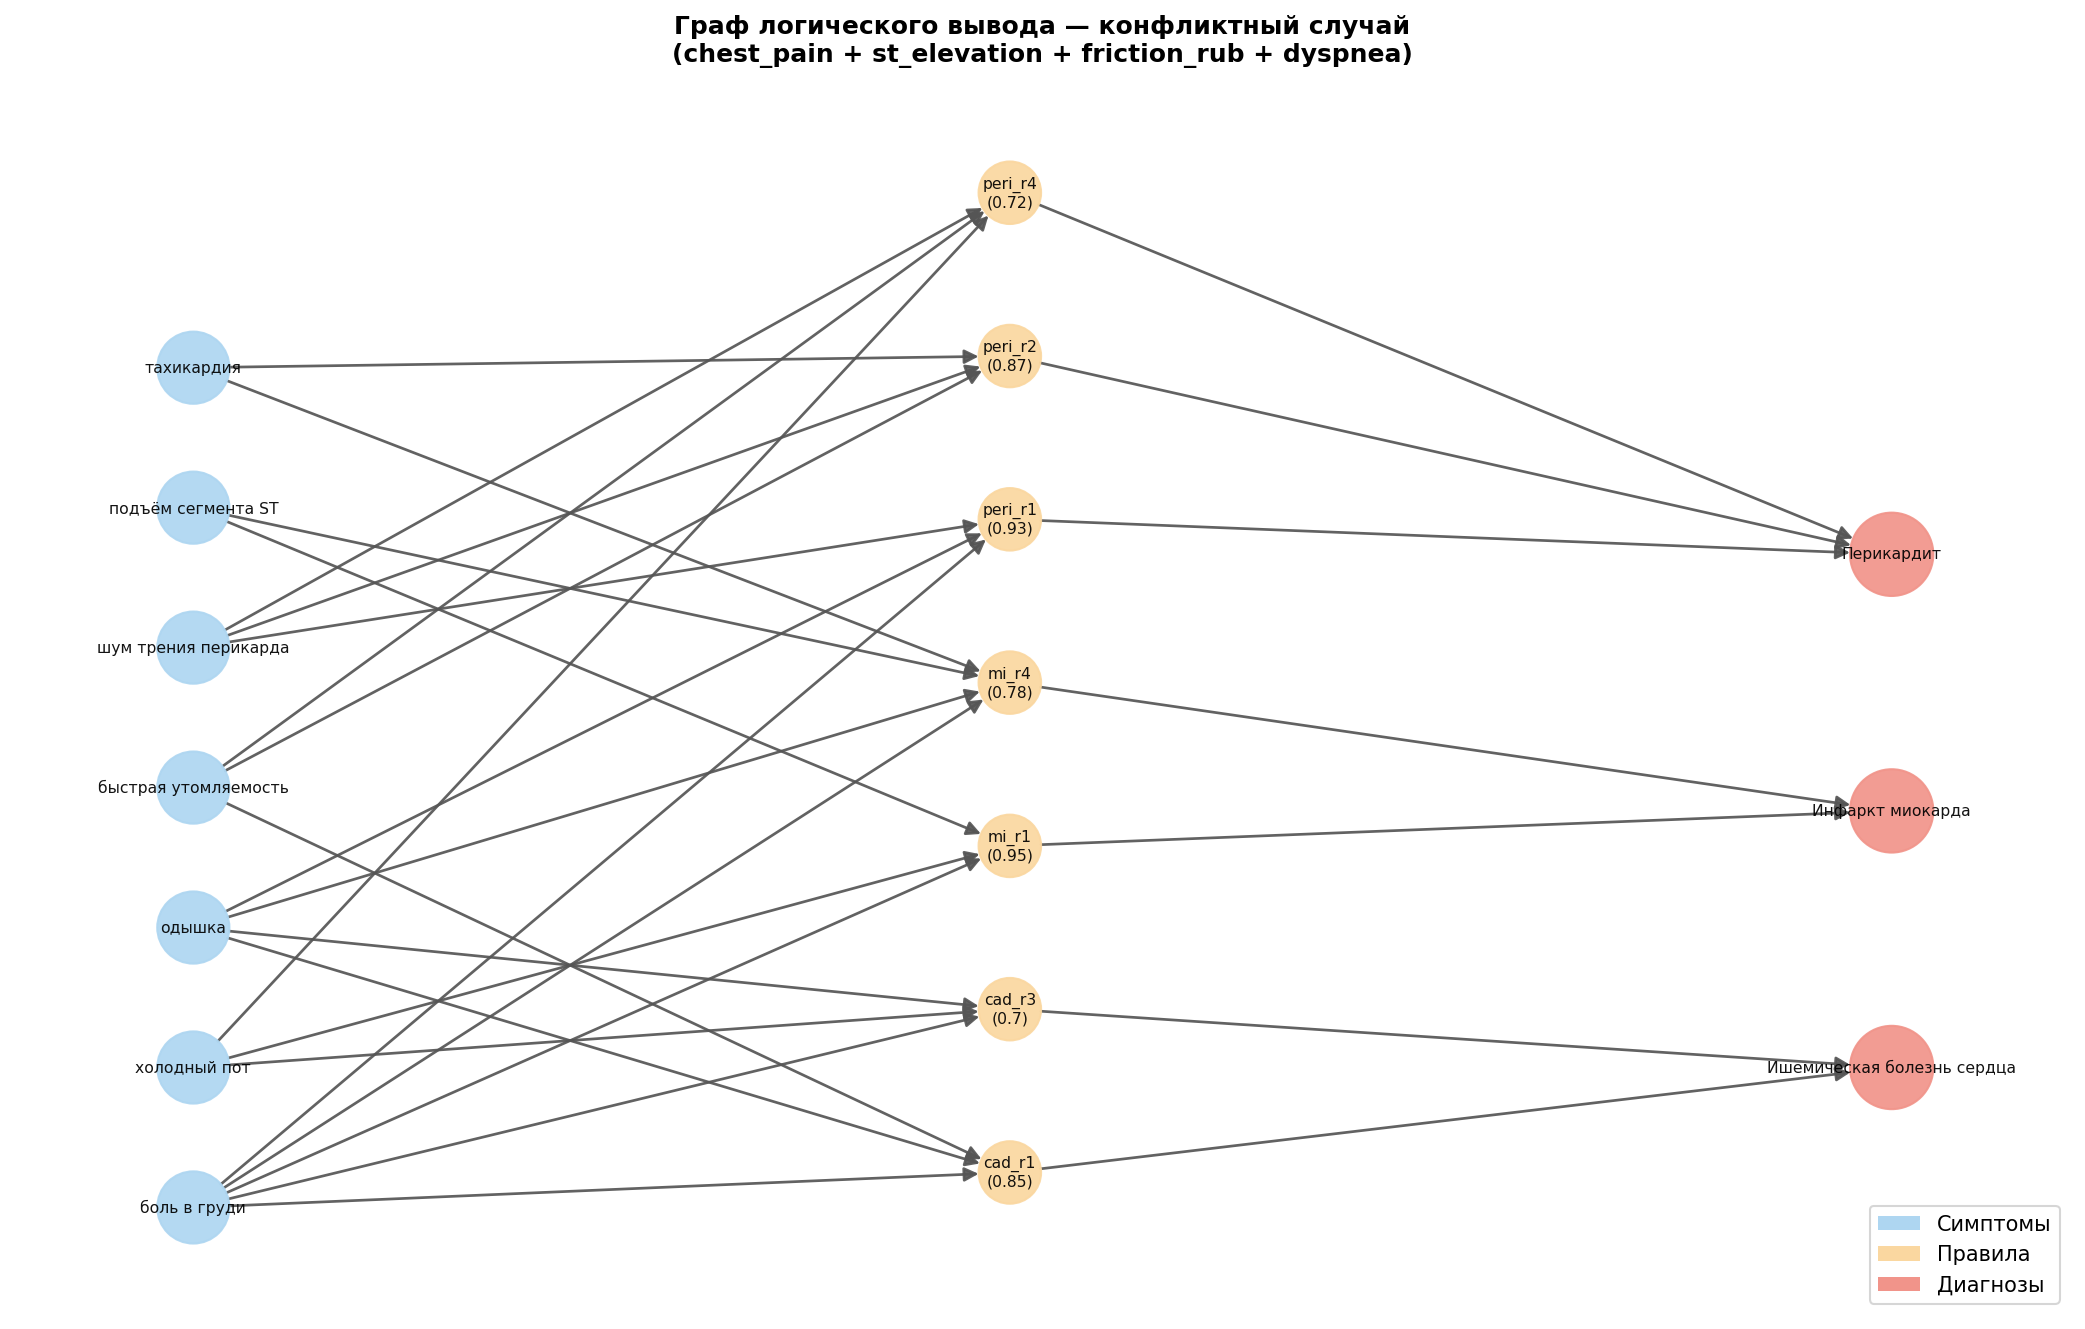
\includegraphics[width=0.95\textwidth]{figures/inference_graph.png}
  \caption{Граф вывода для конфликтного случая. Цвета: симптомы --- голубые, правила --- жёлтые, диагнозы --- лососевые}
  \label{fig:graph}
\end{figure}

\subsection{Дерево первичного триажа}

На рисунке~\ref{fig:tree} представлено дерево решений для экстренного триажа кардиологического пациента. Первый разветвляющий вопрос --- наличие боли в груди; второй уровень проверяет подъём~ST или периферические отёки; третий уровень уточняет специфику нозологии.

\begin{figure}[H]
  \centering
  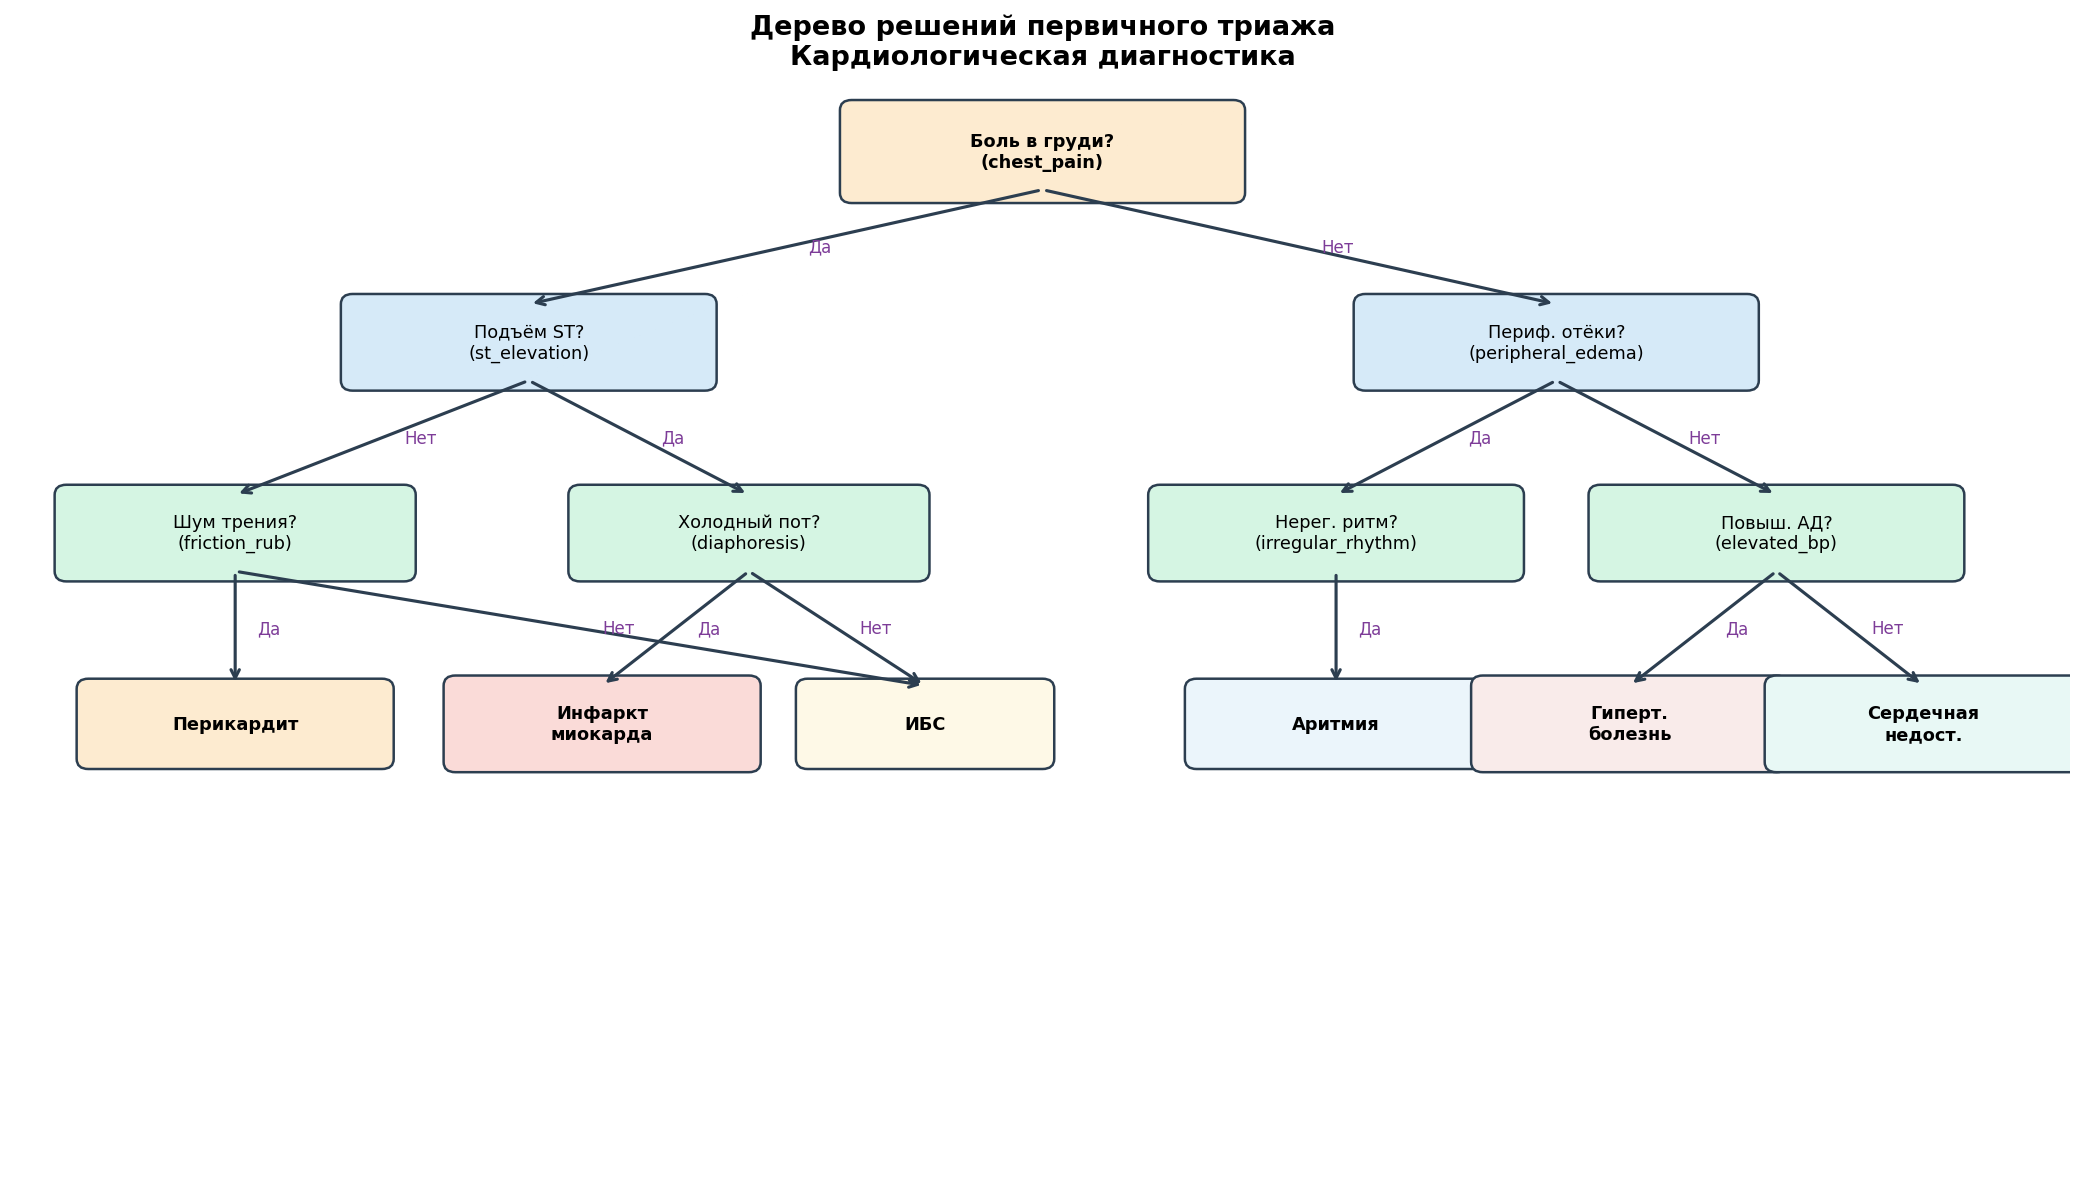
\includegraphics[width=0.97\textwidth]{figures/decision_tree.png}
  \caption{Дерево решений первичного триажа. Диагнозы-листья выделены цветовой кодировкой по степени срочности}
  \label{fig:tree}
\end{figure}

\subsection{ReAct-цикл (12 итераций)}

Агент ReAct моделирует клинический процесс последовательного сбора информации о пациенте М., 58~лет (сценарий острого инфаркта миокарда). На каждой итерации агент:
\begin{enumerate}
  \item \textbf{Perceive} --- принимает текущий набор клинических признаков (с нарастанием числа доступных данных);
  \item \textbf{Reason} --- применяет базу знаний, вычисляет уверенность для всех нозологий, ранжирует диагнозы;
  \item \textbf{Act} --- выбирает клиническое действие: наблюдение, дополнительное обследование или экстренное вмешательство.
\end{enumerate}

На рисунке~\ref{fig:react} отображена динамика уверенности в топ-диагнозе по итерациям. До итерации~6 правила ИМ не активируются из-за отсутствия подъёма~ST; с~итерации~7 уверенность скачкообразно возрастает до~0{,}98 и пересекает порог экстренного действия~(0{,}90), после чего агент переходит к рекомендации ЧКВ.

\begin{figure}[H]
  \centering
  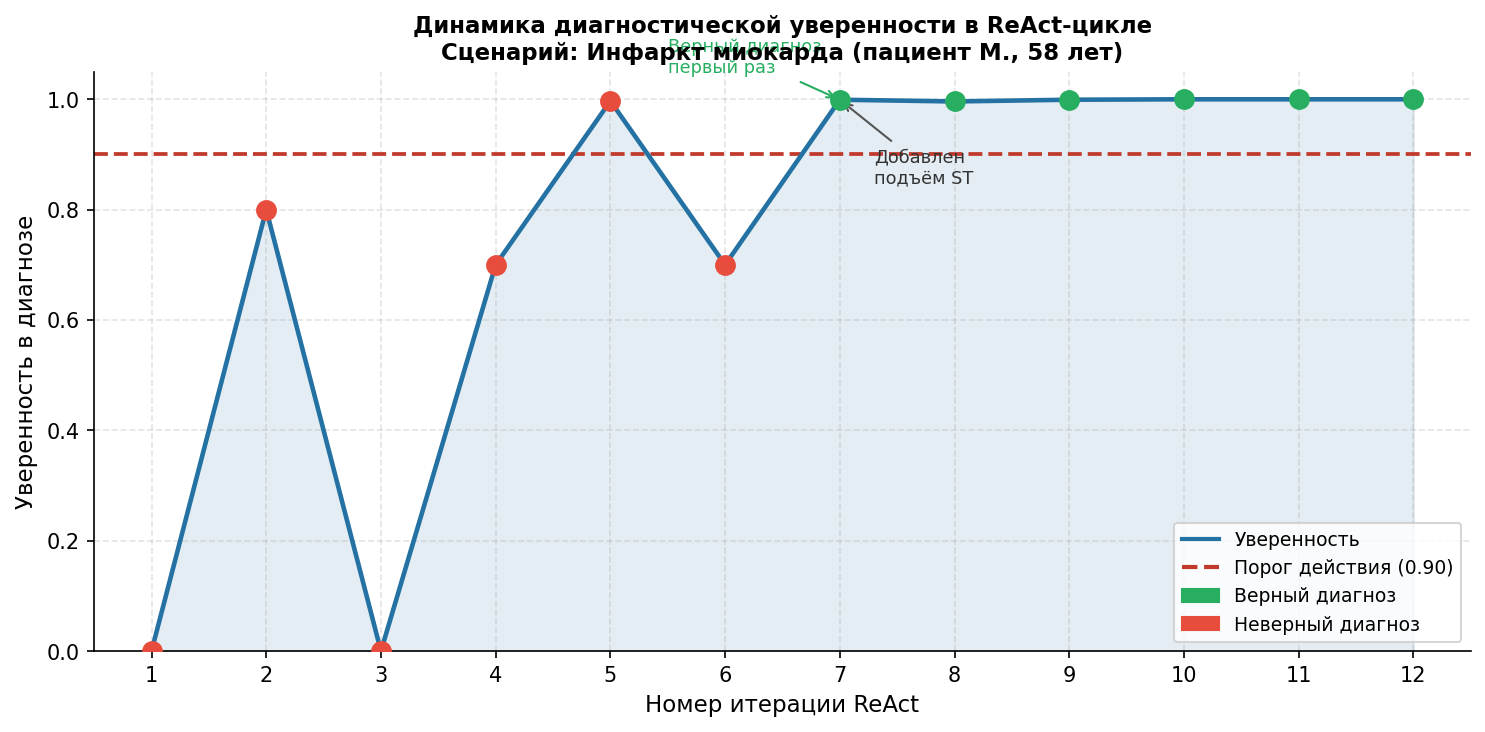
\includegraphics[width=0.90\textwidth]{figures/react_timeline.png}
  \caption{Динамика диагностической уверенности в ReAct-цикле. Красная пунктирная линия --- порог экстренного вмешательства~(0{,}90). Зелёные точки --- итерации с верным диагнозом}
  \label{fig:react}
\end{figure}

Бонусный интерактивный интерфейс реализован в скрипте \texttt{interactive\_cli.py}: пользователь последовательно отмечает симптомы из пронумерованного списка и мгновенно получает ранжированный список диагнозов с уверенностью и рекомендованным клиническим действием.

\section{Заключение}

В работе разработана прототипная экспертная система дифференциальной кардиологической диагностики на основе трёх парадигм логического программирования. База знаний включает 22 диагностических правила, охватывающих 6 нозологий и 15 клинических признаков.

Механизм НЕ-факторов реализован на всех трёх уровнях: через отрицание от неудачи в Prolog, через аннотированные дизъюнкции в ProbLog и через ограничения целостности в ASP. Взаимные исключения инфаркт\,/\,ИБС и перикардит\,/\,СН корректно разрешаются во всех 8 тестовых случаях.

Сравнение ProbLog и ASP на 300 синтетических сценариях показало, что ProbLog обеспечивает более высокую точность (0{,}75--0{,}78 против 0{,}69--0{,}73 для ASP) за счёт мягкого взвешивания свидетельств, тогда как ASP работает быстрее и предпочтителен для систем с жёсткими временными ограничениями.

Эксперимент с~ReAct-агентом продемонстрировал, что 12-итерационный цикл последовательного сбора данных позволяет достичь клинически приемлемого порога уверенности~(${\geq}\,0{,}90$) к~итерации~7, что соответствует реальной практике постановки экстренного диагноза.

% ===============================================================
% СПИСОК ИСПОЛЬЗОВАННЫХ ИСТОЧНИКОВ
% ===============================================================
\clearpage
\addcontentsline{toc}{section}{Список использованных источников}
\renewcommand{\refname}{\normalfont\bfseries\large СПИСОК ИСПОЛЬЗОВАННЫХ ИСТОЧНИКОВ}

\begin{thebibliography}{9}
\sloppy

\bibitem{bib:gost}
ГОСТ~7.32-2017. СИБИД. Отчёт о научно-исследовательской работе. Структура и правила оформления. --- М.: Стандартинформ, 2017.

\bibitem{bib:cardio2021}
Knuuti~J. et al. 2019 ESC Guidelines for the diagnosis and management of chronic coronary syndromes~// European Heart Journal. --- 2020. --- Vol.~41, №~3. --- P.~407--477.

\bibitem{bib:nilsson1986}
Nilsson~N.\,J. Probabilistic logic~// Artificial Intelligence. --- 1986. --- Vol.~28, №~1. --- P.~71--87.

\bibitem{bib:swipl}
Wielemaker~J. et al. SWI-Prolog~// Theory and Practice of Logic Programming. --- 2012. --- Vol.~12, №~1--2. --- P.~67--96.

\bibitem{bib:problog}
De Raedt~L. et al. ProbLog: A probabilistic Prolog and its application in link discovery~// IJCAI-2007. --- 2007. --- P.~2462--2467.

\end{thebibliography}

\end{document}
